\documentclass{standalone}

\usepackage[utf8]{inputenc}
\usepackage{tikz}
\usetikzlibrary{arrows,3d,matrix}

 % see the explanation below
 \makeatletter
 \tikzoption{canvas is xy plane at z}[]{%
   \def\tikz@plane@origin{\pgfpointxyz{0}{0}{#1}}%
   \def\tikz@plane@x{\pgfpointxyz{1}{0}{#1}}%
   \def\tikz@plane@y{\pgfpointxyz{0}{1}{#1}}%
   \tikz@canvas@is@plane
 }
 \makeatother 

\begin{document}
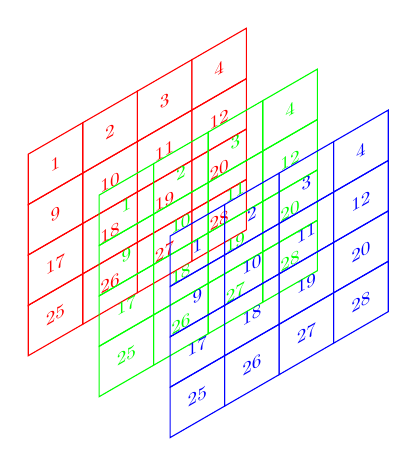
\begin{tikzpicture}[x={(0.866cm,0.5cm)}, y={(-0.866cm,0.5cm)}, z={(0cm,0.8cm)}, scale=0.8]
    \begin{scope}[canvas is xz plane at y=0,transform shape]
      \foreach \ii [count = \xi] in {1,2,3,4}{
        \foreach \jj  [count = \yi]in {1,2,3,4}{
          \pgfmathsetmacro{\nn}{int(\xi+8*\yi-8)}
          \node[red,draw,minimum size=1cm] (n\nn-1) at (\ii,-\jj) {\nn};
        }
      }
    \end{scope}
    \begin{scope}[canvas is xz plane at y=-1.3,transform shape]
      \foreach \ii [count = \xi] in {1,2,3,4}{
        \foreach \jj  [count = \yi]in {1,2,3,4}{
          \pgfmathsetmacro{\nn}{int(\xi+8*\yi-8)}
          \node[green,draw,minimum size=1cm] (n\nn-1) at (\ii,-\jj) {\nn};
        }
      }
    \end{scope}
    \begin{scope}[canvas is xz plane at y=-2.6,transform shape]
      \foreach \ii [count = \xi] in {1,2,3,4}{
        \foreach \jj  [count = \yi]in {1,2,3,4}{
          \pgfmathsetmacro{\nn}{int(\xi+8*\yi-8)}
          \node[blue,draw,minimum size=1cm] (n\nn-1) at (\ii,-\jj) {\nn};
        }
      }
    \end{scope}

  \end{tikzpicture}

  \end{document}
